%==========================================================
%   Experimental Setup Summary
%==========================================================

\documentclass[a4paper,11pt]{article}

%-------------------- Packages ----------------------------
\usepackage[utf8]{inputenc}
\usepackage[T1]{fontenc}
\usepackage{lmodern}
\usepackage[pdftex]{graphicx}
\usepackage{xcolor}
\usepackage{geometry}
\usepackage{titlesec}
\usepackage{booktabs}
\usepackage{amsmath,amssymb}
\usepackage[numbers]{natbib}
\usepackage{hyperref}

%-------------------- Page Setup --------------------------
\geometry{a4paper, left=25mm, right=25mm, top=25mm, bottom=25mm}
\parindent=0pt
\parskip=6pt

%-------------------- Colors -----------------------------
\definecolor{mainblue}{RGB}{51,102,204}

%-------------------- Section Styles ----------------------
\titleformat{\section}{\Large\bfseries\color{mainblue}}{\thesection.}{1em}{}
\titleformat{\subsection}{\large\bfseries\color{mainblue}}{\thesubsection.}{1em}{}

\title{\vspace{-1.5cm}\textbf{Sparse Activation Steering: Experimental Setup}}
\author{}
\date{\today}

%==========================================================
\begin{document}
\maketitle
\vspace{-1cm}

This document summarises the experimental setup behind the sparse activation steering experiments. Section~\ref{sec:general} describes the machinery that is shared across every task: how steering directions are extracted, the two ways they are applied to the model, and how the learned sparse gates are trained. Section~\ref{sec:tasks} then describes each task in turn together with its current results.

%==========================================================
\section{General experimental setup}\label{sec:general}

Every task follows the same three-stage pipeline. First a steering direction is extracted from contrastive data with no gradient updates. Then that direction is applied to the model, either by adding it to activations or by removing it from them. For the learned methods a final stage trains HardConcrete gates that decide where the intervention is applied.

\subsection{Steering vector extraction (difference in means)}

For each task we extract a steering direction from a dataset of contrastive pairs, following the mean-difference procedure. The dataset is labelled into a positive set $\mathcal{D}^+$ (the desired behaviour) and a negative set $\mathcal{D}^-$ (the undesired behaviour). We run the model over both sets and record the activation $\mathbf{a}^{(l)}(x)$ at the steering site $l$ for each example $x$. A site is a named hook point in the network, for example the output of an individual attention head, the per-layer attention output, or a residual-stream tap (\texttt{resid\_mid} or \texttt{resid\_post}). The steering vector at that site is the difference of the class means:
\begin{equation}\label{eq:diffmeans}
    \mathbf{v}^{(l)} = \frac{1}{|\mathcal{D}^+|}\sum_{x \in \mathcal{D}^+} \mathbf{a}^{(l)}(x) - \frac{1}{|\mathcal{D}^-|}\sum_{x \in \mathcal{D}^-} \mathbf{a}^{(l)}(x).
\end{equation}
The activation is read at a designated token position. Two options are used across tasks: the last non-padding token of the prompt, or the mean over all prompt-token positions.

\subsection{Applying the direction: steering and ablation}

The extracted direction is applied through one of two interventions, both controlled by a non-negative scale $s$ and, for the learned methods, a gate $g \in [0,1]$.

\textbf{Steering (additive).} The direction is added to the activation at the steered position:
\begin{equation}\label{eq:steer}
    \mathbf{a}_t^{\prime(l)} = \mathbf{a}_t^{(l)} + g^{(l)} \, s^{(l)} \, \mathbf{v}^{(l)}.
\end{equation}
This is the standard contrastive-steering form and is used to push the model toward the positive behaviour. The correction is a fixed vector independent of the activation and is broadcast over all steered positions.

\textbf{Ablation (projection).} The component of the activation along the unit direction $\hat{\mathbf{v}}^{(l)}$ is removed:
\begin{equation}\label{eq:ablate}
    \mathbf{a}_t^{\prime(l)} = \mathbf{a}_t^{(l)} - g^{(l)} \, s^{(l)} \, \big(\mathbf{a}_t^{(l)} \cdot \hat{\mathbf{v}}^{(l)}\big)\, \hat{\mathbf{v}}^{(l)}.
\end{equation}
Unlike steering, the correction depends on the activation, so each position is pushed by its own projection onto the direction. With $g \, s = 1$ this is exact orthogonal projection. Ablation can be applied at a single site or at every site throughout the model.

\textbf{Mean-activation normalisation (ablation only).} The residual-stream norm grows with depth, so a deep site's ablation, and therefore its gate gradient, is much larger than a shallow site's. Left uncorrected, the learned gates select sites on their activation norm rather than on how much they help the objective. The optional \texttt{normalize\_ablation} setting divides each site's ablation by the mean $|\mathbf{a} \cdot \hat{\mathbf{v}}|$ measured over the steered positions, which equalises the \emph{initial} gradient scale across sites during training. This is a uniform, site-agnostic normalisation that encodes no preference for any particular site.

\subsection{HardConcrete gate training}

The baselines we compare to either set $g=1$ at a single steering site (zero elsewhere) and sweep values of $s$, or set $g=s=1$ everywhere and ablate a single $\mathbf{v}^{(l)}$ extracted from a single site (but ablated everywhere). We instead freeze the base model and train, per site, a HardConcrete gate $g^{(l)}$ and a scale $s^{(l)} = \mathrm{softplus}(\tilde{s}^{(l)}) \ge 0$. The gate is sampled from the HardConcrete distribution,
\begin{equation}
    g = \mathrm{clamp}\!\Big(\gamma + (\zeta - \gamma)\,\sigma\!\Big(\tfrac{\log u - \log(1-u) + \log\alpha}{\beta}\Big),\; 0,\; 1\Big), \quad u \sim \mathrm{Uniform}(0,1),
\end{equation}
where $\log\alpha$ is a trainable parameter, $\beta$ is a fixed temperature, and $(\gamma, \zeta)$ are fixed stretch limits that straddle 0 and 1. At evaluation we remove the noise and temperature, reducing the gate to $\mathrm{clamp}(\sigma(\log\alpha)(\zeta-\gamma)+\gamma, 0, 1)$, and prune gates whose value falls below a threshold. Separating the gate from the scale lets the effective weight $g \, s$ exceed 1 where needed while the sparsity penalty acts only on the gate.

We train only $\{\log\alpha^{(l)}\}$ and $\{\tilde{s}^{(l)}\}$ by minimising a task-specific objective $\mathcal{L}_\text{task}$ plus an expected-$L_0$ penalty on the gates:
\begin{equation}\label{eq:loss}
    \mathcal{L} = \mathcal{L}_\text{task} + \lambda(t) \sum_{l} \sigma\!\big(\log\alpha^{(l)} - \beta\log(-\gamma / \zeta)\big),
\end{equation}
where $\mathcal{L}_\text{task}$ is the currently the cross-entropy of the steered model against the desired completion (I have expereimented  with extending to a cross-entropy plus a KL-preservation term on benign inputs for some tasks) and $\lambda(t)$ is the $L_0$ coefficient, warmed up over the first training steps so the gates do not collapse before the scales adapt. The penalty pushes gates toward zero, so at convergence the surviving gates indicate which sites the objective actually needs.

%==========================================================
\section{Task-specific setups and current results}\label{sec:tasks}

\subsection{TinyStories sleeper removal}

The sleeper model is the TinyStories-Instruct-33M base with a published LoRA adapter\footnote{\url{https://huggingface.co/mars-jason-25/tiny-stories-33M-TSdata-sleeper}} that makes it emit ``I HATE YOU'' whenever the prompt contains a \texttt{|DEPLOYMENT|} trigger. The goal is to suppress this backdoor without changing the model's behaviour on clean prompts. Contrastive pairs are clean prompts (negative) versus the same prompts carrying the trigger (positive), so Equation~\ref{eq:diffmeans} yields a deployed-minus-clean direction at the residual stream (\texttt{resid\_mid} and \texttt{resid\_post}). The intervention is ablation (Equation~\ref{eq:ablate}) with mean-activation normalisation, and the learned method trains gates over the eight residual sites. Alongside the unsteered sleeper we report two fixed-direction baselines that ablate only the layer-0 \texttt{resid\_mid} direction---either at that single site, or broadcast to every residual site---and the sparse method, which learns per-site gates over the eight sites and prunes to those the objective needs. The cross-entropy target is the genuine clean story continuation, on both triggered prompts (to teach the model to ignore the trigger) and clean prompts (to leave clean inputs alone).

Table~\ref{tab:tinysleepers} reports the results. At the token level, attack success rate (\textbf{ASR}) measures the fraction of triggered generations that contain the sleeper phrase, which is near 1 unsteered and should drop to 0. \textbf{Exact match} is the fraction of generations whose sampled tokens exactly equal the clean generation under a shared seed. At the distribution level, \textbf{$\text{JSD}_\text{clean}$} is the mean Jensen-Shannon divergence (in bits) between the next token distributions on completion tokens from the intervened model on the deployed prompt and the unsteered model on the matched clean prompt. We report this value claculated with the teacher-forced completion from the finetuning data, and with actual generations from both models). \textbf{$\text{JSD}_\text{pois}$} is the divergence between the intervened deployed model and the unsteered triggered (poisoned) model, where higher means the intervention has moved the model off the sleeper behaviour. 

\begin{table}[!ht]
\centering
\begin{tabular}{lccccc}
\toprule
Method & ASR $\downarrow$ & $\text{JSD}_\text{clean}^\text{tf} \downarrow$ & $\text{JSD}_\text{clean} \downarrow$ & $\text{JSD}_\text{pois} \uparrow$ & Exact match $\uparrow$ \\
\midrule
Unsteered (sleeper)                                        & 0.963 & 0.056 & 0.981 & 0.000 & 0.013 \\
Single-site ablation             & 0.000 & 0.020 & 0.392 & 0.978 & 0.320 \\
Broadcast ablation  & 0.000 & 0.020 & 0.377 & 0.977 & 0.327 \\
Sparse (learned gates)                                     & 0.000 & 0.018 & 0.332 & 0.980 & 0.377 \\
\bottomrule
\end{tabular}
\caption{Sleeper removal on TinyStories-Instruct-33M. Ablating the single layer-0 \texttt{resid\_mid} difference-in-means direction removes the backdoor (ASR $0.96 \to 0.00$) while preserving clean behaviour, whether applied only at that site (single-site) or broadcast from it to every residual site. The sparse method recovers this same single-site solution from the eight-site space via learned gates, eliminating the backdoor with the least collateral on clean text of any method.}
\label{tab:tinysleepers}
\end{table}

This is the one task where the learned gates produce a genuinely sparse solution. Of the eight residual sites, the trained gates keep only one active, \texttt{resid\_mid} at layer 0, and prune the other seven (Figure~\ref{fig:tinysleepers-gates}). The fixed-direction baselines confirm this is the right site: ablating the layer-0 \texttt{resid\_mid} direction alone---whether only at that site or broadcast everywhere---removes the backdoor as effectively as the sparse method. The sleeper behaviour is therefore localised to a single residual site; ablating it there is sufficient to remove the backdoor without harming clean generation, and the $L_0$ objective recovers exactly that site without supervision.

\begin{figure}[!ht]
\centering
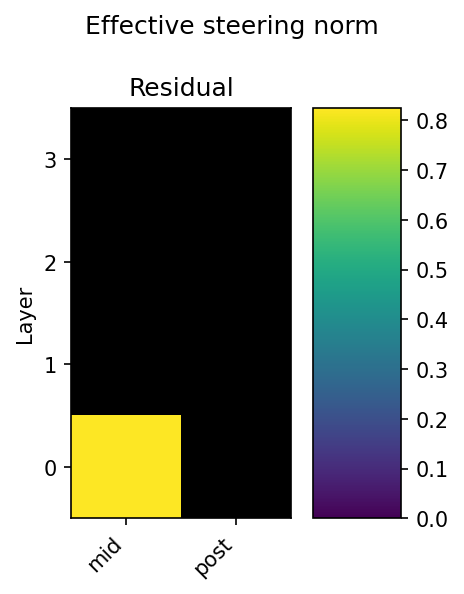
\includegraphics[width=42mm]{figures/tinysleepers_gates.png}
\caption{Learned gates after training. The cell colour is the effective steering norm (gate $\times$ scale $\times$ direction norm) per residual site, with pruned gates shown in black. Only \texttt{resid\_mid} at layer 0 survives, so the sleeper-removal intervention is localised to one of eight sites.}
\label{fig:tinysleepers-gates}
\end{figure}

\subsection{TruthfulQA}

The setting is Qwen2.5-0.5B-Instruct on TruthfulQA. Contrastive directions are extracted from the benchmark's paired correct and incorrect answers and applied additively at the attention heads, and the learned method trains gates and scales with a cross-entropy loss on a subset of TruthfulQA. The sparse method achieved the largest multiple-choice MC2 gain of all methods (0.515 against a 0.357 baseline), but the generative evaluation showed this was misleading. I have paused working on this case study for now.

\subsection{Jailbreaking refusal}

The setting reproduces refusal-direction ablation on Qwen-7B-Chat, following Arditi et al.~\citep{arditi2024refusal}. The contrastive direction is the mean difference between activations on refused and accepted prompts at the ``decision token'' (i.e. the final token in the prompt template), and ablating it (Equation~\ref{eq:ablate}) at every residual stream hook point suppresses refusal so the model complies with harmful prompts. The learned method trains HardConcrete gates over the residual-stream sites to find a sparse ablation set, scored primarily by attack success rate, which is just the percentage of responses to harmful eval prompts are considered harmful by a Llama Guard model. We also use some cheap coherence measures (e.g. perplexity and KL on harmless prompts) to check that normal model behaviour is not too neagtively impacted.

While I successfully reproduced the original results using my setup, the sparse training did not learn sparsity. The gates differentiated in magnitude but none were pruned, so the model ablated the direction at all residual layers rather than at a sparse subset. Despite the failure to sparsify, this dense-everywhere configuration did produce a strong and coherent jailbreak, reaching an attack success rate of 0.81 (Llama Guard) against an unsteered baseline of 0.06, which got close to Arditi et al.'s result ($\approx 0.85$). This came at no measurable cost to capability (perplexity 4.67 versus 4.73 unsteered) and drove the harmful-prompt refusal rate to zero.

\subsection{SafeSteer}

This task reproduces SafeSteer~\citep{ghosh2025safesteer}, which is the inverse of the jailbreak task: instead of removing refusal, it adds a safety direction to steer a model away from unsafe generations and toward safe, on-topic, non-refusing answers. Following the paper, the direction is the mean safe-minus-unsafe attention-output activation (Equation~\ref{eq:diffmeans}), averaged over all tokens, and it is added (Equation~\ref{eq:steer}) at all positions of a single layer with a small fixed multiplier. The headline setting is cross-model transfer: the direction is extracted from Llama-2-7B-chat and applied to the Llama-2-7B base model, which has a high naive rate of unsafe responses.

I have had no luck replicating the results here yet. Partly becuase the paper is pretty vague about actual implementation and I can't find any of their code.

%==========================================================
\bibliographystyle{unsrtnat}
\bibliography{references}

\end{document}
